\documentclass{beamer}

\usepackage{tikz}
\usepackage{tkz-berge}
\usepackage{tkz-graph}

\usetikzlibrary{patterns,arrows,decorations.pathreplacing}

\usepackage{xcolor}
\definecolor{dblue}  {RGB}{20,66,129}

\title{Fractals avoiding Fractal Sets}
\author{Jacob Denson}
\institute{University of British Columbia}

\begin{document}

\maketitle

\begin{frame}
  \frametitle{Examples of Configuration Problems}

\begin{tabular}{p{0.6\textwidth}p{0.4\textwidth}}

\begin{itemize}
     \item How large can a subset of the $\mathbf{R}$ be such that it contains no three term arithmetic progressions?

     \pause
     \item How large can a subset of $\mathbf{R}^d$ be such that the distances between any two points are distinct?

     \pause
     \item How large can a subset of $\mathbf{R}^d$ be such that the angles formed from any three points in $X$ are irrational?
  \end{itemize} &

\begin{itemize}
  \item[]
    %\begin{tikzpicture}
    %    \draw (0,0) -- (1,0);
    %\end{tikzpicture}

  \item[]
    %\begin{tikzpicture}
    %    \draw (0,0) -- (1,0);
    %\end{tikzpicture}

    \item[]
    %\begin{tikzpicture}
    %    \draw (0,0) -- (1,0);
    %\end{tikzpicture}

\end{itemize} \\

\end{tabular}

\end{frame}

\begin{frame}
    \frametitle{Two Observations}

    \begin{itemize}
        \item These are `multi-scale' configurations.
        \pause

        \begin{itemize}
        \item Every open set contains these configurations.
        \pause

        \item Even every set of positive measure has these configurations.
        \pause

        \item We need a `second order' notion of size.
        \pause

        \item We use Hausdorff dimension (Not too technically!).
        \pause
    \end{itemize}

        \item The problems can be stated by avoiding values of a function.
        \pause
        \begin{itemize}
            \item $x,y,z$ is in a three term arithmetic progression if and only if $f(x,y,z) = (x - y) - (y - z) = 0$.
            \pause

            \item The distances between two pairs $x,y$ and $z,w$ are non distinct when $f(x,y;z,w) = d(x,y) - d(z,w) = 0$.
            \pause

            \item The angles formed by three points are irrational when $f(x,y,z) = (x - z)(y - z)/|x-z||y-z| \not \in \cos(\mathbf{Q})$.
        \end{itemize}
    \end{itemize}
\end{frame}

\begin{frame}
    \frametitle{General Results}

    \begin{itemize}
        \item {\bf Configuration Avoidance Problem}: Given $f: [0,1]^{nd} \to \mathbf{R}$, find $X \subset \mathbf{R}^d$ with high Hausdorff dimension such that for any distinct $x_1, \dots, x_n \in X$, $f(x_1, \dots, x_n) \neq 0$.
        \pause

        \item Math\'{e} (2017) proved that if $f$ is a polynomial of degree $r$, we can find $X$ with dimension $d/r$.
        \pause

        \item Pramanik and Fraser (2018) proved that if $f$ is smooth and nonsingular, we can find $X$ with dimension $d/(n-1)$.
    \end{itemize}
\end{frame}

\begin{frame}
    \frametitle{Increasing the Difficulty}

    \begin{center}
     \Huge {\it What if the zero sets of the function are also fractals...}
    \end{center}
\end{frame}

%\begin{frame}
%    \frametitle{The Avoidance Problem}

%        \begin{itemize}

%            \item Our method naturally considers an equivalent setup.

%            \item {\bf Fractal Avoidance Problem}: Given $Y \subset \mathbf{R}^{nd}$, find $X \subset \mathbf{R}^d$ such that $X^n \cap Y \subset \Delta$, where $\Delta = \{ x: x_i = x_j\ \text{for some $i,j$} \}$.

%            \item Equivalent by setting $Y = f^{-1}(0)$, or $f = \mathbf{I}_{Y^c}$.

%            \item Our method only uses the structure of the zero set, not $f$.
%        \end{itemize}
%\end{frame}

\begin{frame}
    \frametitle{Main Result}

    \begin{theorem}
        If the zero set of $f$ is $\alpha$ dimensional, we can find $X$ with
        %
        \[ \dim_{\mathbf{H}}(X) = \frac{nd - \alpha}{n - 1} = \frac{\text{codim}_{\mathbf{H}}(f^{-1}(0))}{n - 1} \]
        %
        such that for any distinct $x_1, \dots, x_n \in X$, $f(x_1, \dots, x_n) \neq 0$.
    \end{theorem}

    \pause

    \begin{itemize}
        \item Extension of Pramanik and Fraser's result (2018), who proved the case where $f$ is smooth and nonsingular, so $f^{-1}(0)$ is a smooth surface of dimension $nd - d$.
        \pause

        \item Shows smoothness is only needed to get a bound on the Hausdorff dimension. Not needed anywhere else.
    \end{itemize}
\end{frame}

\begin{frame}
    \frametitle{Applications}

    \begin{center}
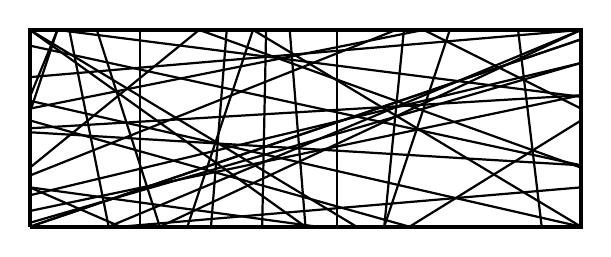
\begin{tikzpicture}[scale=0.5]
%\draw[help lines] (0,0) grid (14,5);

\draw[ultra thick] (0,0) -- (14,0) -- (14,5) -- (0,5) -- (0,0);

\draw[thick] (0,3.3) -- (0.7,5);
\draw[thick] (0,2.7) -- (9.642,0);
\draw[thick] (0,2.5) -- (14,3.34);
\draw[thick] (0,2.4) -- (14,1.56);
\draw[thick] (0,1) -- (2.3,0);
\draw[thick] (0,0) -- (14,4.76);
\draw[thick] (0,0.8) -- (14,4.16);
\draw[thick] (2.8,0) -- (2.8,5);
\draw[thick] (1.7,5) -- (3.3,0);
\draw[thick] (0,1.5) -- (4.3,5);
\draw[thick] (0,3) -- (10,5);
\draw[thick] (4,0) -- (5.66666,5);
\draw[thick] (1,5) -- (2,0);

\draw[thick] (0,2.9) -- (0.7,5);
\draw[thick] (0,3.2) -- (14,0);
\draw[thick] (0,0.4) -- (14,3.34);
\draw[thick] (0,4.6) -- (14,1.56);
\draw[thick] (0,1) -- (7.3,0);
\draw[thick] (0,0) -- (14,4.76);
\draw[thick] (0,0.1) -- (14,4.16);
\draw[thick] (7.8,0) -- (7.8,5);
\draw[thick] (0,5) -- (8.3,0);
\draw[thick] (0,1.3) -- (9.3,5);
\draw[thick] (0,3.8) -- (14,5);
\draw[thick] (9,0) -- (10.66666,5);
\draw[thick] (0,5) -- (7,0);

\draw[thick] (14,3.3) -- (0.7,5);
\draw[thick] (14,2.7) -- (9.642,0);
\draw[thick] (14,2.5) -- (14,3.34);
\draw[thick] (14,2.4) -- (14,1.56);
\draw[thick] (14,1) -- (2.3,0);
\draw[thick] (14,0) -- (14,4.76);
\draw[thick] (14,0.8) -- (14,4.16);
\draw[thick] (14,5) -- (3.3,0);
\draw[thick] (14,1.5) -- (4.3,5);
\draw[thick] (14,3) -- (10,5);
\draw[thick] (14,0) -- (5.66666,5);
\draw[thick] (14,5) -- (2,0);

\draw[thick] (7,0) -- (6.6,5);
\draw[thick] (9,0) -- (9.5,5);
\draw[thick] (13,0) -- (12.4,5);
\draw[thick] (4.6,0) -- (5,5);
\draw[thick] (5.9,0) -- (6,5);
\end{tikzpicture}
\end{center}

    \begin{itemize}
        \item More robust result of Pramanik and Fraser, showing that we can `thicken' or `thin' the zero set of our function with stable effects on the Hausdorff dimension of $X$.
        \pause

        \item Uncountable unions of regular sets are allowed!
        \pause

        \item General results in this direction assume $f$ is regular. We don't assume anything about $f$.
    \end{itemize}
\end{frame}

\begin{frame}
    \frametitle{Applications}

    \begin{itemize}
        \item Given a continuous $\gamma: [0,1] \to \mathbf{R}^d$, finding $X \subset [0,1]$ such that $\gamma(x), \gamma(y), \gamma(z)$ do not form an `arithmetic progression' on the curve, in the sense that
        %
        \[ (\gamma(x) - \gamma(y)) - (\gamma(y) - \gamma(z)) = 0 \]
        %
        Pramanik and Fraser can avoid smooth curves. We can now avoid any curve given a Hausdorff dimension bound. Potentially even a Hilbert curve?
        \pause

        \item Given a subset $Y$ of $\mathbf{R}^d$ with dimension $\alpha$, we can find a subset $X$ of dimension $d - \alpha$ such that $X + X$ and $X - X$ are disjoint from $Y$. I hope to extend this shortly with the additional criterion that the set $X$ we construct is a rational vector space, so for instance $X + X + X$ is disjoint from $Y$. Then $X \oplus Y$ is a full dimensional subspace of $\mathbf{R}$.
    \end{itemize}
\end{frame}

\begin{frame}
    \frametitle{The Method}

    \begin{columns}

    \column{0.1\textwidth}

    \column{0.7\textwidth}
    {\Huge Two key ideas: }
    \pause

     \begin{itemize}
        \item {\Large Discretization of Scales.}
        \pause

        \item {\Large Random Disection.}
     \end{itemize}

     \end{columns}
\end{frame}

\begin{frame}
    \frametitle{Discretization of Scales: Intuition}

    \begin{itemize}
        \item Every number in the Cantor set has a trinary expansion which does not contain the digit 1.
        \pause

        \item We can view this as a `fine scale property', since it involves the infinite digit expansion of a number.
        \pause

        \item Scale discretization changes fine-scale configurations into an infinite sequence of discrete configurations which are easier to achieve.
        \pause

        \item {\bf Discrete Problem}: Given $X_n$, find $X_{n+1}$ such that no element of $X_{n+1}$ has $1$ as the $n$'th digit in it's expansion.
    \end{itemize}
\end{frame}

\begin{frame}
    \frametitle{Discretization of Scales}

    \begin{center}
    \includegraphics[scale=0.15]{CantorSet.png}
    \end{center}

    \begin{itemize}

        \item We take $X = \lim X_n$, where $X_{n+1}$ is obtained from $X_n$ by interval disection avoiding a discretized problem.
        \pause

        \item {\bf Discrete Configuration Problem}: If $f(x_1, \dots, x_n) = 0$ for $x_1, \dots, x_n \in X_n$, then some $x_i$ and $x_j$ occur in a common interval.
        \pause

        \item If the interval lengths in $X_n$ tend to zero as $n \to \infty$, and $x_1, \dots x_n \in X$ have $f(x_1, \dots, x_n) = 0$, then there is $i,j$ such that $|x_i - x_j| = o(1)$, so $x_i = x_j$.
    \end{itemize}
\end{frame}

\begin{frame}
    \frametitle{Discrete Scale Problem}

    \begin{center}
    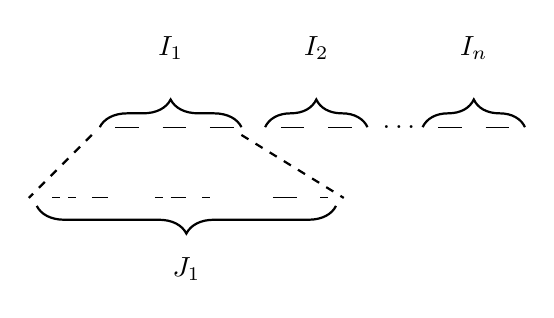
\begin{tikzpicture}[scale=0.1]
        \draw (-6,0) -- (-3,0);
        \draw (0,0) -- (3,0);
        \draw (6,0) -- (9,0);

        \draw (15,0) -- (18,0);
        \draw (21,0) -- (24,0);

        \node at (30,0) {$\dots$};

        \draw (35,0) -- (38,0);
        \draw (41,0) -- (44,0);

        \draw [thick, decorate,decoration={brace,amplitude=10pt},xshift=0.4pt,yshift=-0.4pt](-8,0) -- (10,0) node[black,midway,yshift=1cm] {$I_1$};

        \draw [thick, decorate,decoration={brace,amplitude=10pt},xshift=0.4pt,yshift=-0.4pt](13,0) -- (26,0) node[black,midway,yshift=1cm] {$I_2$};

        \draw [thick, decorate,decoration={brace,amplitude=10pt},xshift=0.4pt,yshift=-0.4pt](33,0) -- (46,0) node[black,midway,yshift=1cm] {$I_n$};

        \draw[thick, dashed] (-9,-1) -- (-17, -9);
        \draw[thick, dashed] (10,-1) -- (23,-9);

        \draw (-15,-9) -- (-15,-9);
        \draw (-14,-9) -- (-13,-9);
        \draw (-12,-9) -- (-11,-9);
        \draw (-9,-9) -- (-7,-9);

        \draw (-1,-9) -- (0,-9);
        \draw (1,-9) -- (3,-9);
        \draw (5,-9) -- (6,-9);

        \draw (14,-9) -- (17,-9);
        \draw (20,-9) -- (21,-9);

        \draw [thick, decorate,decoration={brace,amplitude=10pt,mirror},xshift=0.4pt,yshift=-0.4pt](-16,-10) -- (22,-10) node[black,midway,yshift=-0.8cm] {$J_1$};
    \end{tikzpicture}
    \end{center}

    \begin{itemize}
    \item For technical reasons, we only disect subsets of $X_n$ at a time.
    \pause

    \item {\bf Discrete Configuration Problem:} Given disjoint unions of intervals sets $I_1, \dots, I_n$, find $J_1 \subset I_1, \dots, J_n \subset I_n$ such that the cartesian product of the $J_k$ avoids $f^{-1}(0)$.
    \pause

        \item Using a queueing procedure, if the subsets we choose cover our entire set infinitely often, we still avoid the finte scale configuration. See Pramanik and Fraser (2018) for the same technique applied to their problem.
    \end{itemize}
\end{frame}

\begin{frame}
    \frametitle{Exploiting Randomness}

    \begin{center}
    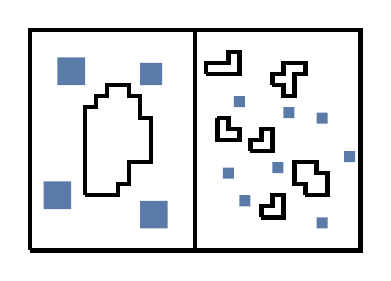
\begin{tikzpicture}[scale=0.7]
%\draw[help lines] (0,0) grid (6,4);

% Y1
\draw[ultra thick] (1,1) -- (1,2.6) -- (1.2,2.6) -- (1.2,2.8) -- (1.4,2.8) -- (1.4,3) -- (1.8,3) -- (1.8,2.8) -- (2,2.8) -- (2,2.4) -- (2.2,2.4) -- (2.2,1.6) -- (1.8,1.6) -- (1.8,1.2) -- (1.6,1.2) -- (1.6,1) -- (1,1);

% X1
% Blue: 88 122 160
\fill[fill=dblue!70] (0.5,3.5) -- (1,3.5) -- (1,3) -- (0.5,3) -- (0.5,3.5);
\fill[fill=dblue!70] (0.25, 0.75) -- (0.25, 1.25) -- (0.75,1.25) -- (0.75, 0.75) -- (0.25,0.75);
\fill[fill=dblue!70] (2,0.4) -- (2.5,0.4) -- (2.5,0.9) -- (2,0.9) -- (2,0.4);
\fill[fill=dblue!70] (2,3) -- (2,3.4) -- (2.4,3.4) -- (2.4,3) -- (2,3);

% Frame
\draw[ultra thick] (0,0) -- (3,0) -- (3,4) -- (0,4) -- (0,0);
\draw[ultra thick] (3,0) -- (6,0) -- (6,4) -- (3,4) -- (3,0);

% Y2
\draw[ultra thick] (3.2,3.2) -- (3.8,3.2) -- (3.8,3.4) -- (3.8,3.6) -- (3.6,3.6) -- (3.6,3.4) -- (3.2,3.4) -- (3.2,3.2);
\draw[ultra thick] (4,1.8) -- (4,2) -- (4.2,2) -- (4.2,2.2) -- (4.4,2.2) -- (4.4,1.8) -- (4,1.8);
\draw[ultra thick] (5,1) -- (5,1.2) -- (4.8,1.2) -- (4.8,1.6) -- (5.2,1.6) -- (5.2,1.4) -- (5.4,1.4) -- (5.4,1) -- (5,1);
\draw[ultra thick] (4.4,3) -- (4.4,3.2) -- (4.6,3.2) -- (4.6,3.4) -- (5,3.4) -- (5,3.2) -- (4.8,3.2) -- (4.8,2.8) -- (4.6,2.8) -- (4.6,3) -- (4.4,3);
\draw[ultra thick] (4.2,0.6) -- (4.2,0.8) -- (4.4,0.8) -- (4.4,1) -- (4.6,1) -- (4.6,0.6) -- (4.2,0.6);
\draw[ultra thick] (3.4,2.4) -- (3.6,2.4) -- (3.6,2.2) -- (3.8,2.2) -- (3.8,2) -- (3.4,2) -- (3.4,2.4);

% X2
\fill[fill=dblue!70] (3.8,0.8) -- (3.8,1) -- (4,1) -- (4,0.8) -- (3.8,0.8);
\fill[fill=dblue!70] (3.7, 2.6) -- (3.9,2.6) -- (3.9,2.8) -- (3.7,2.8) -- (3.7,2.6);
\fill[fill=dblue!70] (5.7, 1.6) -- (5.9,1.6) -- (5.9,1.8) -- (5.7,1.8) -- (5.7,1.6);
\fill[fill=dblue!70] (4.4,1.4) -- (4.4,1.6) -- (4.6,1.6) -- (4.6,1.4) -- (4.4,1.4);
\fill[fill=dblue!70] (3.5, 1.3) -- (3.7,1.3) -- (3.7,1.5) -- (3.5,1.5) -- (3.5,1.3);
\fill[fill=dblue!70] (5.2, 2.3) -- (5.4,2.3) -- (5.4,2.5) -- (5.2,2.5) -- (5.2,2.3);
\fill[fill=dblue!70] (4.6,2.4) -- (4.6,2.6) -- (4.8,2.6) -- (4.8,2.4) -- (4.6,2.4);
\fill[fill=dblue!70] (5.2,0.4) -- (5.4,0.4) -- (5.4,0.6) -- (5.2,0.6) -- (5.2,0.4);

\end{tikzpicture}
\end{center}

    \begin{itemize}
        \item How do we prove the discrete scale argument?
        \pause

        \item Aside from the Hausdorff dimension of $f^{-1}(0)$, we have little knowledge of it's structure.
        \pause

        \item Random choices of the $J_k$ avoid $f^{-1}(0)$ effectively.

        \pause
        \item We obtain that for all but $o(1)$ of these sections, $J_k$ contains a length $1/N^\beta$ section, where $\beta = d(nd - \alpha)/(n - 1)$. This ratio gives the Hausdorff dimension bound $(nd-\alpha)/(n-1)$ for $X$.
    \end{itemize}
\end{frame}

\begin{frame}
    \frametitle{Conclusion}

    {\Huge So What's Next?}
\end{frame}

\begin{frame}
    \frametitle{Extension to Hausdorff Dimension}

    \begin{itemize}
        \item I left out something in the statement of my theorem.
        \pause

        \item Our theorem needs the assumption that $f^{-1}(0)$ is the countable union of sets with {\it lower} Minkowski dimension $\alpha$.
        \pause

        \item Our techniques `should' work when $f^{-1}(0)$ has {\it Hausdorff dimension} $\alpha$.
        \pause

        \item We are trying to use hyperdyadic coverings to obtain this.
    \end{itemize}
\end{frame}

\begin{frame}
    \frametitle{Analogies with Hypergraphs}

    \begin{itemize}
        \item Partition $I_1, \dots, I_n$ into length $1/N^\beta$ sections. Form a hypergraph whose vertices are the sections, and add a hyperedge between $K_1 \subset I_1, \dots, K_n \subset I_n$ if $K_1 \times \dots \times K_n$ intersects $f^{-1}(0)$.
        \pause

        \item Our discrete configuration problem reduces to finding independant sets in hypergraphs.
        \pause

        \item The method we use essentially generalizes Turan's theorem to hypergraphs, and is tight?
        \pause

        \item We are looking to using other methods on hypergraphs to improve the bound when $f^{-1}(0)$ has certain structural properties.
    \end{itemize}
\end{frame}

\begin{frame}
    \frametitle{You're Interested in Learning More?}

Read these to find out more about configuration problems:

    \begin{itemize}
            \item Read Keleti (1999) for a simple use of scale discretization on a particular configuration avoidance problem.
            \pause
            \item Read M\'{a}th\'{e} (2017) for a construction where $f$ is assumed to be a polynomial of bounded degree.
            \pause
            \item Read Pramanik and Fraser (2018) for a general construction where $f$ is smooth and nonsingular. We generalize their work.
            \pause
    \end{itemize}

    Thanks for listening!
\end{frame}

\end{document}